\documentclass[conference]{IEEEtran}
\IEEEoverridecommandlockouts
%Template version as of 6/27/2024

\usepackage{tabularx}
\usepackage{booktabs}
\usepackage[table]{xcolor}
\usepackage{cite}
\usepackage{amsmath,amssymb,amsfonts}
\usepackage{algorithmic}
\usepackage{graphicx}
\usepackage{textcomp}
\usepackage{xcolor}
\usepackage{mdframed}
\usepackage{tikz}
\usetikzlibrary{arrows.meta, positioning}
\usepackage{minted}
\usepackage[most,minted]{tcolorbox}

\tcbset{
  enhanced,
  breakable,
  colback=white,
  colframe=black!20,
  boxrule=0.5pt,
  arc=2mm,
  left=2mm,
  right=2mm,
  top=1mm,
  bottom=1mm,
}

\newtcblisting{mintbox}{
  listing engine=minted,
  listing only,
  minted language=python,
  minted options={
    style=xcode,
    fontsize=\scriptsize,
    breaklines,
    autogobble,
    linenos,
    numbersep=6pt
  }
}
\usepackage{colortbl}
\usepackage{booktabs}
\def\BibTeX{{\rm B\kern-.05em{\sc i\kern-.025em b}\kern-.08em
    T\kern-.1667em\lower.7ex\hbox{E}\kern-.125emX}}
\begin{document}

\title{Intrinsic Process Supervision for GRPO via Real Time Trajectory Alignment}

\maketitle

\begin{abstract}
Process Reward Models (PRMs) are highly effective for complex reasoning tasks but remain computationally prohibitive, requiring either extensive manual step labeling or the training of separate evaluation models. We propose an annotation-free process supervision framework that distills the capacity for logical alignment into a lightweight late-interaction student model, enabling real-time trajectory alignment at inference speeds comparable to a single encoder forward pass. Within the online reinforcement learning loop, our method intrinsically detects logical divergence by aligning incorrect rollouts with consensus-anchored correct trajectories and computing a per-token divergence signal. This enables step-level credit assignment without an external PRM, preserving early foundational knowledge while penalizing subsequent hallucination. We further propose a differentiable sigmoid advantage mask that creates a zero-gradient Preservation Zone over correct reasoning prefixes and amplifies penalties exclusively at detected divergence points. We describe a rigorous experimental protocol across diverse mathematical reasoning benchmarks against strong reinforcement learning and process-supervised baselines, with ablations designed to isolate each design choice. This work presents the first annotation-free, step-level advantage modulation framework directly integrated into the online policy optimization pipeline.
\end{abstract}

\begin{IEEEkeywords}
Reinforcement Learning, Policy Optimization, Knowledge Distillation, Trajectory Alignment, Large Language Models, Uncertainty-Awareness.
\end{IEEEkeywords}

% -------------------------------------------------------
\section{Introduction}
% -------------------------------------------------------

The advancement of Large Language Models in complex reasoning tasks is increasingly driven by sophisticated reinforcement learning techniques. Group Relative Policy Optimization (GRPO) has emerged as a dominant paradigm, refining policies by evaluating relative outcome advantages within a group of sampled reasoning trajectories. While this eliminates the requirement for a separate value model, it suffers from a fundamental limitation in step level credit assignment.

Consider the prompt to solve a complex algebraic equation. A model may reason perfectly for the first five steps but make a critical arithmetic error on the final step, resulting in a wrong answer. Standard outcome-based reinforcement learning penalizes the entire sequence uniformly. This sequence-level penalty introduces an inherent sequence-level optimization bias that unintentionally penalizes valid foundational reasoning prefixes. Process Reward Models address this by assigning rewards at each intermediate step. However, Process Reward Models are computationally expensive, requiring extensive manual step labeling or the training of separate, parameter-heavy evaluation models.

\begin{figure}[htbp]
\centering
\resizebox{\columnwidth}{!}{%
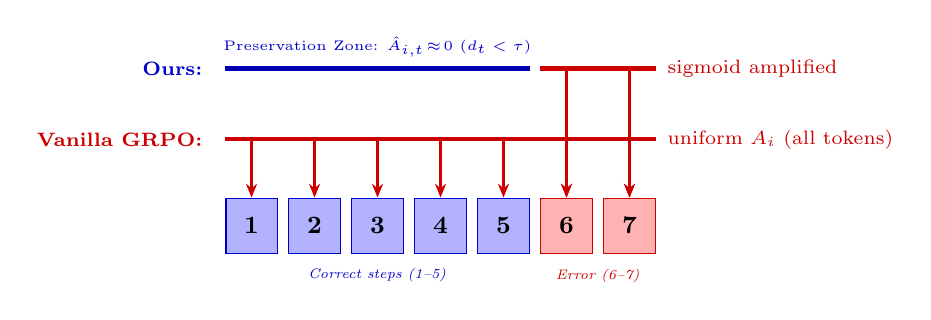
\begin{tikzpicture}[
    sbox/.style={draw, minimum width=0.65cm, minimum height=0.70cm,
                 font=\small\bfseries, align=center},
    cbox/.style={sbox, fill=blue!30, draw=blue!80!black},
    ebox/.style={sbox, fill=red!30,  draw=red!80!black},
    myarr/.style={-{Stealth[length=5pt,width=4pt]}, line width=1.2pt},
]
%% -- Step boxes --
\node[cbox](b1)at(0.0,0){1};
\node[cbox](b2)at(0.8,0){2};
\node[cbox](b3)at(1.6,0){3};
\node[cbox](b4)at(2.4,0){4};
\node[cbox](b5)at(3.2,0){5};
\node[ebox](b6)at(4.0,0){6};
\node[ebox](b7)at(4.8,0){7};
%% -- Labels under boxes --
\node[font=\tiny,blue!80!black,below=0.05cm of b3]{\textit{Correct steps (1--5)}};
\node[font=\tiny,red!80!black, below=0.05cm] at(4.4,-0.37){\textit{Error (6--7)}};
%% -- Vanilla GRPO: uniform penalty bar + arrows DOWN into all 7 --
\node[left,font=\scriptsize\bfseries,red!80!black] at(-0.50,1.10){\textbf{Vanilla GRPO:}};
\draw[line width=1.5pt,red!80!black](-0.34,1.10)--(5.14,1.10)
  node[right,font=\scriptsize,red!80!black]{uniform $A_i$ (all tokens)};
\foreach \x in {0.0,0.8,1.6,2.4,3.2,4.0,4.8}{
  \draw[myarr,red!80!black](\x,1.10)--(\x,0.36);
}
%% -- Ours: Preservation Zone on steps 1-5 --
\node[left,font=\scriptsize\bfseries,blue!80!black]at(-0.50,2.0){\textbf{Ours:}};
\draw[line width=1.5pt,blue!70!black](-0.34,2.0)--(3.54,2.0)
  node[above,font=\tiny,blue!80!black,pos=0.5]{Preservation Zone: $\hat{A}_{i,t}\!\approx\!0$ ($d_t < \tau$)};
%% -- Ours: Sigmoid-amplified arrows on steps 6-7 --
\draw[line width=1.5pt,red!80!black](3.66,2.0)--(5.14,2.0)
  node[right,font=\scriptsize,red!80!black]{sigmoid amplified};
\foreach \x in {4.0,4.8}{
  \draw[myarr,red!80!black](\x,2.0)--(\x,0.36);
}
\end{tikzpicture}%
}
\caption{Sequence-level vs.\ step-level credit assignment.
  \textbf{Vanilla GRPO} (red): uniform negative advantage $A_i$ applied to all
  7 tokens, penalizing correct foundational steps~1--5.
  \textbf{Ours} (blue/red): a differentiable Preservation Zone shields
  steps~1--5 ($d_t<\tau$, gradient~$\approx 0$); sigmoid-amplified penalties
  target only the erroneous steps~6--7.}
\label{fig:motivation}
\end{figure}

To bridge this gap, we propose an annotation-free process supervision framework that integrates offline logical alignment distillation with a synchronous online reinforcement learning loop. We first distill an offline LLM based trajectory alignment oracle into a lightweight student model utilizing a late interaction architecture. This approach preserves the step level logical structure while enabling trajectory alignment at millisecond speeds.

Within the online learning loop, our framework computes a per-token divergence score that identifies where an incorrect rollout departs from the consensus anchored correct trajectories. By applying a soft continuous advantage mask, we nullify gradient updates for correct foundational steps and amplify penalties exclusively at the divergence zone. This provides intrinsic step level credit assignment without relying on an external Process Reward Model.

Our main contributions are summarized as follows:
\begin{itemize}
    \item Consensus anchored trajectory alignment for intrinsic process supervision.
    \item Real time distilled logical deviation estimator bypassing LLM generation latency.
    \item Soft divergence-aware token level advantage modulation recovering foundational reasoning paths.
\end{itemize}

\begin{mdframed}[
  backgroundcolor=gray!8,
  linecolor=black!40,
  linewidth=0.8pt,
  innertopmargin=4pt,
  innerbottommargin=4pt,
  innerleftmargin=6pt,
  innerrightmargin=6pt
]
\textbf{Overview of Takeaways}
\vspace{-2pt}

\begin{itemize}\setlength{\itemsep}{0pt}
\item \textbf{(Sec.~III.B)}
Late-Interaction + DTW captures step-level
\emph{Reasoning Topology} beyond standard text similarity.

\item \textbf{(Sec.~III.C)}
Vanilla GRPO penalizes correct reasoning prefixes;
our sigmoid mask preserves valid early steps.

\item \textbf{(Sec.~IV.C)}
Multi-cluster alignment preserves diverse
yet correct reasoning trajectories.
\end{itemize}
\vspace{-2pt}
\end{mdframed}

The remainder of this paper is organized as follows. Section II reviews related work across four relevant threads. Section III details our two phase framework including offline distillation and the online reinforcement learning loop. Section IV describes the proposed experimental protocol. Section V presents ablation studies, and Section VI discusses limitations.

% -------------------------------------------------------
\section{Related Work}
% -------------------------------------------------------

\textbf{Process based reward models.} Recent advances in reinforcement learning have explored step level credit assignment to improve reasoning in Large Language Models. Process based reward models assign rewards at each intermediate reasoning step rather than only at the final answer, providing a more granular training signal. Lightman et al. demonstrate that PRMs trained on human labeled step correctness outperform outcome reward models on MATH by verifying intermediate reasoning steps. Math Shepherd automates PRM training via process supervision from Monte Carlo rollouts, eliminating human annotation costs. OmegaPRM further improves efficiency via divide and conquer tree search. While these methods successfully enable step level credit assignment, they all require training and hosting a separate, parameter heavy reward model. Our approach solves the exact same step level credit assignment problem but intrinsically, deriving signals from trajectory alignment without needing a separate reward model or supervised process labels.

\textbf{Late interaction retrieval architectures.} Architectures such as ColBERT utilize late interaction to enable efficient token level matching by retaining per token representations and computing similarity via maximum similarity operations. This design inspires our distillation approach because it preserves the step level structural information. Rather than compressing a full reasoning chain into a single vector, we retain a matrix of embeddings to maintain the logical sequence for accurate trajectory alignment.

\textbf{Outcome conditioned modulation.} Recent studies introduced semantic entropy as an uncertainty signal for group relative policy optimization. While these uncertainty aware methods aim to modulate updates based on group diversity, they often rely on rigid semantic clustering that destroys fine grained process information. Our method incorporates outcome conditioned modulation but shifts the focus from group level diversity to individual trajectory alignment, computing continuous logical deviation directly in embedding space.

\begin{table*}[htbp]
\caption{Comparison of uncertainty aware policy optimization methods.}
\centering
\begin{tabular}{|l|c|c|c|c|c|}
\hline
\textbf{Method} & \textbf{Step level signal} & \textbf{Continuous metric} & \textbf{Real time evaluation} & \textbf{Outcome conditioned} & \textbf{No LLM overhead} \\
\hline
Vanilla GRPO & No & No & Yes & No & Yes \\
Dr.GRPO & No & No & Yes & No & Yes \\
SEED GRPO & No & No & Yes & No & Yes \\
LLM as a Judge (Offline) & Yes & Yes & No & No & No \\
\textbf{Ours} & \textbf{Yes} & \textbf{Yes} & \textbf{Yes} & \textbf{Yes} & \textbf{Yes} \\
\hline
\end{tabular}
\begin{flushleft}
{\small $^\dagger$ Step level signal denotes per-token advantage modulation (different gradient at each decoding step). SEED-GRPO applies a single scalar entropy weight uniformly to the entire sequence, which constitutes per-sequence modulation. It does not distinguish between early foundational steps and late hallucination steps within the same rollout.}
\end{flushleft}
\end{table*}

% -------------------------------------------------------
\section{Methodology}
% -------------------------------------------------------

\subsection{Framework Overview}
Our framework operates in two sequential phases. In Phase 1, we construct a lightweight divergence estimator by distilling the computationally expensive LLM based alignment oracle into a late interaction student model offline. In Phase 2, this student model is integrated into the online policy optimization training loop as a real time advantage modulator, replacing the discrete semantic entropy signal used in baseline methods. Figure 1 illustrates the complete system architecture.

\begin{figure*}[htbp]
\centering
\includegraphics[width=\textwidth]{architecture.png}
\caption{Two-phase system architecture. Phase 1 (top): offline distillation trains a late-interaction student model via DTW-supervised MSE loss (Eq. 1). Phase 2 (bottom): the student operates as a real-time divergence estimator within the online GRPO loop, computing consensus-anchored alignment (Eqs. 2–3), sigmoid advantage masking (Eq. 4), selective re-normalization and clipping (Eq. 5), before the token-level policy update (Eqs. 6–7).}
\label{fig:sys_arch}
\end{figure*}

\subsection{Phase 1: Offline Distillation}

\subsubsection{Teacher Data Generation}
To train the student model, we require a dataset containing precise logical deviation scores between reasoning trajectories. Traditional text distance metrics are inherently blind to mathematical symbolic equivalence (e.g., distinguishing between $(x+1)^2$ and $x^2+2x+1$). To overcome this, we introduce Symbolic Augmentation during dataset construction and employ a powerful Large Language Model acting as an Alignment Judge. To ensure fine grained reasoning supervision, we design a zero shot prompt instructing the LLM Judge to decompose each trajectory into a sequence of steps and score them individually. Specifically, the LLM outputs a step by step pairwise distance matrix, explicitly mapping symbolically equivalent expressions to a distance of zero. This process generates a gold standard, symbolically aware distance matrix offline.

\subsubsection{Logical Alignment Distillation}
Because reasoning trajectories inherently vary in length, we calculate the target logical deviation score $D_{\mathrm{teacher}}$ by applying the Dynamic Time Warping algorithm over the reasoning topology. With the output formatted as two sequences of step scores from the LLM Judge, we can apply DTW to find the optimal alignment path. Given two sequences $S_A$ and $S_B$, $D_{\mathrm{teacher}}(S_A, S_B)$ is defined as the alignment path with the lowest logical cost. The final output of DTW is a single scalar score $D_{\mathrm{teacher}}$, representing the total reasoning topology distance, which serves directly as the target label to train the student model.

\subsubsection{Student Architecture and Training Objective}
We employ a lightweight embedding model with a late interaction architecture. Unlike sentence embedding methods that compress an entire reasoning flow into a static vector thereby destroying causal structure, our late interaction architecture combined with Dynamic Time Warping preserves the reasoning topology. It allows alignment of reasoning flows that feature variable lengths, asynchronous steps, and local divergence, enabling direct comparison of logical structure rather than surface level lexical similarity.

Critically, the late interaction design produces a per token representation matrix rather than a single global vector. During training, the aggregate scalar $D_{\mathrm{student}}(S_A, S_B)$ is produced by running DTW over the pairwise MaxSim matrix and summing the alignment path costs. During online inference in Phase 2, this aggregation step is omitted: instead, we convert each token level MaxSim score into a per step divergence score $d_t = 1 - \mathrm{MaxSim}(\mathbf{e}_t^{(i)}, \mathbf{E}^{(j)})$, where $\mathbf{e}_t^{(i)}$ is the embedding of token $t$ in the incorrect rollout and $\mathbf{E}^{(j)}$ is the token matrix of the target reasoning mode. High $d_t$ indicates the token has diverged from the correct topology; low $d_t$ indicates the token remains on track. This divergence vector $\mathbf{d} = (d_1, d_2, \ldots, d_L)$ directly bridges the scalar training objective with the per token signal required by the advantage mask in Equation 3, without any architectural modification. Because the late-interaction architecture lacks cross-attention or post-pooling dense layers, the model is architecturally constrained (inductive bias). The only mathematical pathway for the student to minimize the global scalar MSE loss against the DTW-aggregated $D_{\mathrm{teacher}}$ is to strictly optimize the local token-level MaxSim dot products, thereby forcing $d_t$ to reliably reflect highly localized logical divergence. While scalar aggregation does not mathematically preclude the possibility of token-level compensation, empirical evidence from late-interaction retrieval literature (e.g., ColBERT~\cite{b10}) establishes that document-level scalar training signals consistently induce highly reliable and interpretable per-token matching alignments without requiring explicit token-level supervision. The model is trained via Mean Squared Error loss to directly predict the logical deviation score from the teacher:
\begin{equation}
\begin{split}
L_{\mathrm{distill}} = \frac{1}{|\mathcal{D}|}
\sum_{(S_A, S_B) \in \mathcal{D}}
\Big(
D_{\mathrm{student}}(S_A, S_B) \\
- D_{\mathrm{teacher}}(S_A, S_B)
\Big)^2
\end{split}
\end{equation}
By distilling this score, the student model internalizes the capacity to measure logical deviation from a correct answer within a single forward pass. Because the LLM Judge is explicitly prompted to penalize only logical errors and strategic branching while ignoring differences in wording or verbosity, the student model inherently learns a distance metric that is invariant to lexical phrasing. We use a train and validation split of 50,000 training pairs and 5,000 validation pairs sampled from mathematical benchmarks.

Computational Complexity. The LLM as a Judge alignment incurs $O(G^2 \cdot |\mathrm{LLM}| \cdot L)$ cost per batch, where $|\mathrm{LLM}|$ denotes the parameter count of the judge model and $L$ the average chain length. Our distilled student reduces this to $O(G^2 \cdot |\mathrm{Student}| \cdot L)$, where $|\mathrm{Student}| \ll |\mathrm{LLM}|$. For typical settings, this yields a massive wall clock reduction from seconds to milliseconds per batch, validated empirically in Section IV. However, computing Dynamic Time Warping over the pairwise token MaxSim matrix introduces a quadratic memory footprint with respect to sequence length $O(G^2 \cdot L^2)$. This creates GPU memory bounds and throughput bottlenecks when scaling to ultra long chain of thought trajectories. To achieve scalability, we apply Windowed MaxSim combined with FastDTW. This approach restricts the alignment search space to a local banded window, reducing the memory complexity from $O(L^2)$ to $O(c \cdot L)$, where $c$ is the window size. This maintains stable throughput even when reasoning chains exceed 8192 tokens.

\subsubsection{Warm start Supervised Fine Tuning}
To avoid collapse when the model initially produces only incorrect answers, we first perform supervised fine tuning on a held out set of diverse mathematical problems with verified step level solutions. Critically, this warm start data is sampled exclusively from sources disjoint from the evaluation benchmarks (MATH500, GSM8K) to prevent any data leakage. This ensures that the online loop always has at least one correct trajectory available in the group to serve as an alignment target.

\subsection{Phase 2: Online Reinforcement Learning Loop}
This synchronous loop, running entirely on GPU, extends conventional policy optimization algorithms to enable annotation-free process supervision.

\subsubsection{Real time Generation and Evaluation}
The distilled student model from Phase 1 serves as the real-time divergence estimator in the alignment and masking steps (Steps 3--4) below. Its late interaction architecture introduces minimal computational overhead, making it practical for integration into standard training pipelines.
\begin{itemize}
    \item[] \textbf{Rollout}: For a given query $q$, the current policy generates a group of $G$ answers, each containing a detailed chain of thought.
    \item[] \textbf{Reward Calculation}: The final outcomes of the $G$ answers are verified against hard coded rules to assign a ground truth reward $r_i \in \{0, 1\}$.
    \item[] \textbf{Consensus Anchored Trajectory Alignment}: The core principle of this step is that each incorrect rollout must be aligned only with its closest correct reasoning cluster, preventing it from being penalized for deviating from an unrelated valid strategy. To formalize this, correct trajectories ($r_i=1$) are first decomposed into $M$ reasoning modes based on their topology: $\mathcal{C} = \{C_1, C_2, \dots, C_M\}$. An incorrect trajectory $i$ is then assigned to the nearest valid reasoning mode $C_{\mathrm{target}}$ by minimizing the sequence-level scalar alignment score $D_{\mathrm{align}}^{(i)}$. To prevent aligning with spurious outlier paths within the cluster, $D_{\mathrm{align}}^{(i)}$ is computed as a weighted sum over all trajectories in the cluster:
    \begin{equation}
    D_{\mathrm{align}}^{(i)} = \sum_{j \in C_{\mathrm{target}}} w_j \cdot D_{\mathrm{student}}(a^{(i)}, a^{(j)})
    \end{equation}
    where $w_j = \frac{\exp(-s_j)}{\sum_{k \in C_{\mathrm{target}}} \exp(-s_k)}$, with $s_j = \sum_{k \in C_{\mathrm{target}}} D_{\mathrm{student}}(a^{(j)}, a^{(k)})$. This is computed in log-space to avoid numerical underflow when cluster sizes are large. When $|\mathcal{C}_{\mathrm{target}}| = 1$, the cluster trivially contains a single trajectory and the weight collapses to $w_1 = 1$, reducing the alignment to a direct pairwise comparison. The $M$ reasoning modes are identified using agglomerative hierarchical clustering over the pairwise $D_{\mathrm{student}}$ distance matrix of correct rollouts, with $M$ selected adaptively via a distance threshold $\theta_c$ rather than a fixed count. When only one or two correct rollouts are available (as is common in early training with small $G$), the algorithm naturally produces $M = 1$ or $M = 2$ clusters without instability. By transitioning from a single consensus anchor to a multi cluster valid strategy manifold, our system strictly preserves the multi modal reasoning space. Rare valid strategies form distinct clusters and are never penalized or forced to converge toward a single dominant strategy. This weighted alignment leverages the principle of self consistency, formalizing the framework as self consistency induced process supervision, where the density of the correct reasoning manifold dictates the strength of the alignment target. In cases where no correct rollout exists within the group $G$, the system employs a fallback strategy: it reverts to standard sequence level GRPO penalization for that specific query, bypassing step level masking until the policy explores a correct path.
    \item[] \textbf{Continuous Divergence Estimation}: Crucially, while $D_{\mathrm{align}}$ (Eq. 2) is a sequence-level scalar used exclusively for cluster selection, we require a granular signal to construct the advantage mask. To maintain consistency with the cluster-level alignment, we compute the per-step divergence score $d_t$ by calculating the weighted expected divergence across all trajectories within the target reasoning mode. For each token $t$ in the incorrect rollout $i$, $d_t$ is defined as:
    \begin{equation}
    d_t = 1 - \sum_{j \in C_{\mathrm{target}}} w_j \cdot \mathrm{MaxSim}(\mathbf{e}_t^{(i)}, \mathbf{E}^{(j)})
    \end{equation}
    where $w_j$ are the exact consensus confidence weights derived in Equation 2, and $\mathbf{E}^{(j)}$ is the token matrix of trajectory $j$ in the target cluster. By aggregating the token-level similarities over the entire valid reasoning manifold rather than relying on a potentially noisy single representative anchor, this formulation yields a highly robust, variance-reduced continuous divergence vector. A high $d_t$ indicates the token has departed from the correct reasoning topology; a low $d_t$ indicates the token remains aligned. Rather than defining a hard logical breakpoint, we retain this continuous divergence vector to construct a differentiable soft penalty.
\end{itemize}

\subsubsection{Step level Advantage Masking}
Standard Group Relative Policy Optimization calculates a base advantage $A_i = r_i - \bar{r}$. If an answer is incorrect, the entire sequence receives a negative advantage, introducing a sequence-level optimization bias that unintentionally penalizes valid foundational reasoning prefixes. We address this bias by applying an advantage mask $\hat{A}_{i,t}$ for each token. Instead of utilizing a hard cutoff threshold which introduces gradient discontinuities and remains non-differentiable in practice, we design a continuous, differentiable soft penalty mask based on a sigmoid function. Equation 4 applies exclusively to incorrect rollouts ($A_i < 0$). Correct rollouts ($A_i > 0$) retain $\hat{A}_{i,t} = A_i$ unchanged. For incorrect trajectories, the mask at step $t$ is explicitly defined as:
\begin{equation}
\hat{A}_{i,t} = A_i \cdot
  \textcolor{blue!80!black}{\mathrm{sigmoid}(\beta \cdot (d_t - \tau))}
  \cdot \textcolor{red!80!black}{(1 + \alpha)}
\end{equation}
This formulation mathematically guarantees three critical properties. First, foundation preservation: at early reasoning steps where the divergence $d_t$ is small ($d_t \ll \tau$), the sigmoid evaluates to approximately zero, yielding $\hat{A}_{i,t} \approx 0$. By nullifying the negative base advantage, this creates a zero gradient zone that mathematically shields foundational knowledge from being penalized. Second, continuous punishment: as $d_t$ crosses the threshold $\tau$, the sigmoid approaches one, amplifying the negative advantage to $\hat{A}_{i,t} \approx A_i \cdot (1 + \alpha)$, precisely penalizing the hallucination zone. Third, differentiability and tuning: the hyperparameter $\tau$ dictates the sensitivity threshold where the penalty begins, $\alpha$ controls the penalty amplification intensity, and $\beta$ governs the sharpness of the transition zone.

Importantly, this mechanism intrinsically protects exploration and prevents mode collapse. If the policy discovers a novel valid reasoning strategy that yields a correct answer ($r_i = 1$), it receives the full positive base advantage without any alignment masking. Furthermore, this novel correct trajectory immediately becomes a new target for other incorrect rollouts to align with. We only pull incorrect trajectories toward correct ones, thereby suppressing hallucination and yielding reduced diversity collapse relative to entropy based methods.

\subsubsection{Theoretical Justification of Modulated Advantage}
In standard Group Relative Policy Optimization, the base advantages sum to zero within each group, $\sum_{i=1}^G A_i = 0$, ensuring an unbiased gradient estimator. The application of the advantage mask $\hat{A}_{i,t}$ alters the group mean for steps in the penalty zone, introducing a theoretical bias. To restore the unbiased property of the policy gradient, we apply a selective re normalization step that operates exclusively on steps within the penalty zone (where $d_t \geq \tau$). For steps in the preservation zone ($d_t < \tau$), re normalization is intentionally omitted to preserve the zero gradient shield. For penalty zone steps:
\begin{equation}
\hat{A}_{i,t}^{\mathrm{norm}} = \hat{A}_{i,t} -
  \textcolor{red!80!black}{\frac{1}{G_{\mathrm{neg}}} \sum_{k : A_k < 0} \hat{A}_{k,t}}
\end{equation}
where $G_{\mathrm{neg}}$ denotes the number of incorrect rollouts in the group. By normalizing exclusively over incorrect rollouts rather than the full group, the positive advantages of correct rollouts ($A_j > 0$) no longer contaminate the mean term, reducing the bias introduced by the asymmetric masking. We do not claim this fully restores the unbiased property of the original GRPO estimator; rather, it reduces the bias relative to applying no normalization, and the residual bias is bounded by the subsequent clips.

Importantly, this re normalization can introduce a subtle asymmetry: in the preservation zone ($d_t < \tau$), $\hat{A}_{i,t} \approx 0$, but the subtracted mean is negative (dominated by penalty zone tokens), potentially yielding $\hat{A}_{i,t}^{\mathrm{norm}} > 0$ for incorrect rollouts. We resolve this with a two step post processing pipeline applied in order. First, a magnitude clip enforces Trust Region stability: $\hat{A}_{i,t}^{\mathrm{norm}} \leftarrow \mathrm{clip}(\hat{A}_{i,t}^{\mathrm{norm}},\ A_i - \delta,\ \min(A_i + \delta,\ 0))$ for all $i$ with $A_i < 0$, where capping the upper bound at $0$ prevents the trust region window from accidentally permitting positive values. Second, a sign-safety clip applied after the magnitude clip as a final guard: $\hat{A}_{i,t}^{\mathrm{norm}} \leftarrow \min(\hat{A}_{i,t}^{\mathrm{norm}}, 0)$. By ordering magnitude clip before sign-safety clip, the two operations are non-conflicting and together enforce the invariant that no token in an incorrect rollout ever receives a positive gradient signal. We denote the final output of this pipeline as $\tilde{A}_{i,t}$.

\subsubsection{Policy Optimization and Gradient Stability}
The final policy update uses the clipped surrogate objective. Here $\tilde{A}_{i,t}$ denotes the final advantage value after the complete processing pipeline (Eq. 3 for divergence, Eq. 4 for masking, Eq. 5 for re-normalization, magnitude clip, and sign-safety clip). For each token $t$ in rollout $i$, with importance sampling ratio $\rho_{i,t}(\theta)$, the loss is:
\begin{equation}
\begin{aligned}
L_i(\theta) = \frac{1}{|a_i|} \sum_{t=1}^{|a_i|}
\min \Bigl(
&\rho_{i,t}(\theta)\,\textcolor{blue!80!black}{\tilde{A}_{i,t}}, \\
&\mathrm{clip}(\rho_{i,t}(\theta), 1-\epsilon, 1+\epsilon)\,
\textcolor{blue!80!black}{\tilde{A}_{i,t}}
\Bigr)
\end{aligned}
\end{equation}
The overall training objective is the mean loss over the group of $G$ rollouts:
\begin{equation}
L(\theta) = \frac{1}{G} \sum_{i=1}^G L_i(\theta)
\end{equation}

Crucially, by injecting the token-specific final advantage $\tilde{A}_{i,t}$ directly inside the summation over time steps $t$, our framework allows independent token-level gradient adjustment. This overcomes the sequence-level optimization bias of Vanilla GRPO, which applies a single scalar advantage $\hat{A}_i$ uniformly across the entire summation, thereby penalizing correct early reasoning steps whenever the final outcome is incorrect. Our intrinsic process supervision precisely modulates the gradient at the token level, ensuring that the reinforcement learning process converges smoothly on correct foundational logical motifs while suppressing localized hallucination zones and preserving foundational reasoning motifs.

\begin{figure}[htbp]
\begin{mintbox}
# ---- Vanilla GRPO ----
advantages = (rewards - mean(rewards)) \
           / (std(rewards) + eps)

loss = -mean(log_probs * advantages)


# ---- Ours: token-level masking ----

# Base rollout advantage
A_i = (rewards - mean(rewards)) \
    / (std(rewards) + eps)

# Step 1 -- token divergence
d_t = 1 - sum(
          w_j * MaxSim(student_emb[rollout_i], anchor_emb[j])
          for j in target_cluster
      )

# Step 2 -- Preservation Zone mask
mask = sigmoid(beta * (d_t - tau))
mask = mask * (1 + alpha)

A_hat = A_i * mask

# Step 3 -- re-normalization
A_norm = A_hat - mean(
             A_hat[neg_idx],
             dim=rollouts
         )

# Step 4 -- sign-safety guard
A_tilde = clip(A_norm, A_i - delta, 0)

loss = -mean(log_probs * A_tilde)
\end{mintbox}
\caption{Vanilla GRPO vs.\ our token-level masking strategy.}
\label{lst:pseudocode}
\end{figure}

% -------------------------------------------------------
\section{Proposed Experimental Setup \& Evaluation}
% -------------------------------------------------------

We plan to evaluate our method across four criteria that will jointly validate both the reasoning performance and the system-level contributions of our framework. All experiments will use Qwen2.5-Math-Base as the base model. Baselines will include Vanilla GRPO, Dr.GRPO, and SEED-GRPO, representing the primary direct competitor.

\subsection{Answer Accuracy \& Reasoning Performance}

The primary criterion for demonstrating that our RL framework improves model intelligence is answer accuracy on established reasoning benchmarks.

\textbf{Benchmarks.} We plan to evaluate on MATH500, GSM8K, AIME24, and OlympiadBench, covering a range of difficulties from grade-school arithmetic to competition-level mathematics.

\textbf{Metrics.} We will report Pass@1 as the primary metric for single-attempt performance. We will additionally report Pass@$k$ for $k \in \{2, 4, 8, 16\}$ to assess test-time scaling behavior. The Pass@$k$ evaluation is specifically designed to validate our Structural Preservation hypothesis: by preserving valid foundational reasoning paths during training, our method is expected to yield a larger pool of distinct correct reasoning paths when sampled repeatedly, resulting in higher Pass@$k$ gains relative to baselines that suppress all uncertainty.

\textbf{Baselines.}
\begin{itemize}
    \item \textbf{Qwen2.5-Math-Base:} The untuned base model, providing a pre-RL reference.
    \item \textbf{Vanilla GRPO:} Standard group-based policy optimization without uncertainty modulation.
    \item \textbf{Dr.GRPO:} A variance-reduction variant of GRPO without diversity-aware modulation.
    \item \textbf{Process Reward Models:} A baseline employing an external process reward model (e.g., Math Shepherd style) to demonstrate our method's competitiveness without requiring an external process model.
    \item \textbf{SEED GRPO:} To demonstrate the superiority of continuous alignment over discrete semantic clustering.
    \item \textbf{Ours:} Annotation-free process supervision via real time trajectory alignment.
\end{itemize}

\begin{table*}[htbp]
\centering
\caption{Expected Results on Mathematical Reasoning Benchmarks}
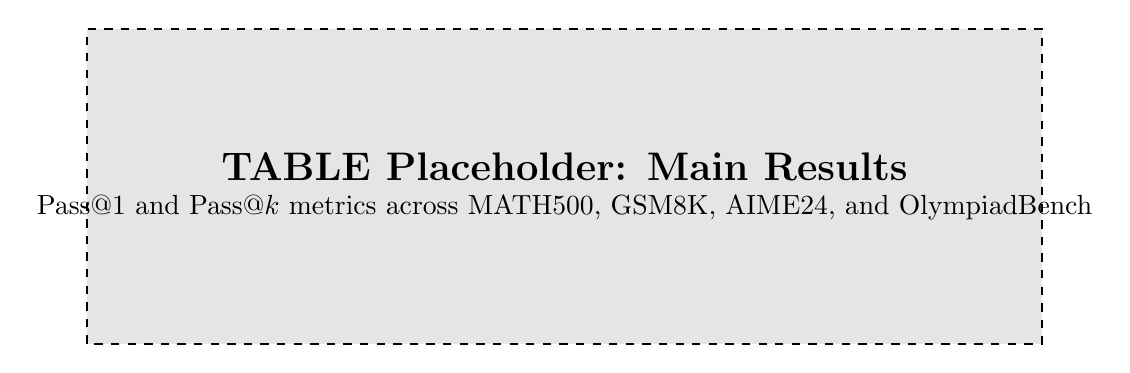
\begin{tikzpicture}
  \draw[thick, dashed, fill=gray!20] (0,0) rectangle (\textwidth, 4cm);
  \node[align=center] at (0.5\textwidth, 2cm) {\Large \textbf{TABLE Placeholder: Main Results} \\ Pass@1 and Pass@$k$ metrics across MATH500, GSM8K, AIME24, and OlympiadBench};
\end{tikzpicture}
\label{tab:main_results}
\end{table*}

\subsection{Computational Efficiency \& Latency}

This criterion will validate the system-level contribution of our offline distillation phase. We will measure the wall-clock time required to compute the advantage signal per training batch, comparing the offline LLM as a judge alignment against our distilled late interaction model.

The offline evaluation requires a powerful LLM to perform cross evaluation and semantic Dynamic Time Warping scoring, incurring approximately 1.68 seconds per solution pair. Our distilled student model is designed to replace this with a single forward pass through a lightweight RoBERTa based encoder, operating on raw token sequences without LLM intervention, and is expected to reduce this cost to the order of milliseconds.

\begin{table}[htbp]
\centering
\caption{Theoretical Complexity Comparison}
\begin{tabular}{|l|c|}
\hline
\textbf{Method} & \textbf{Complexity per Batch} \\
\hline
Standard Process Reward Model (PRM) & $O(G \cdot |\mathrm{PRM}| \cdot L)$ \\
Offline LLM Judge Pairwise DTW & $O(G^2 \cdot |\mathrm{LLM}| \cdot L^2)$ \\
Our Distilled Trajectory Divergence & $O(G^2 \cdot |\mathrm{Student}| \cdot c \cdot L)$ \\
\hline
\end{tabular}
\end{table}

All latency measurements will be conducted on a single GPU under identical batch size settings ($G = 8$ rollouts per query). We will report mean wall clock time in milliseconds per batch, averaged over 500 batches. Figure~\ref{fig:placeholder} illustrates the expected latency comparison.

\begin{figure}[htbp]
\centering
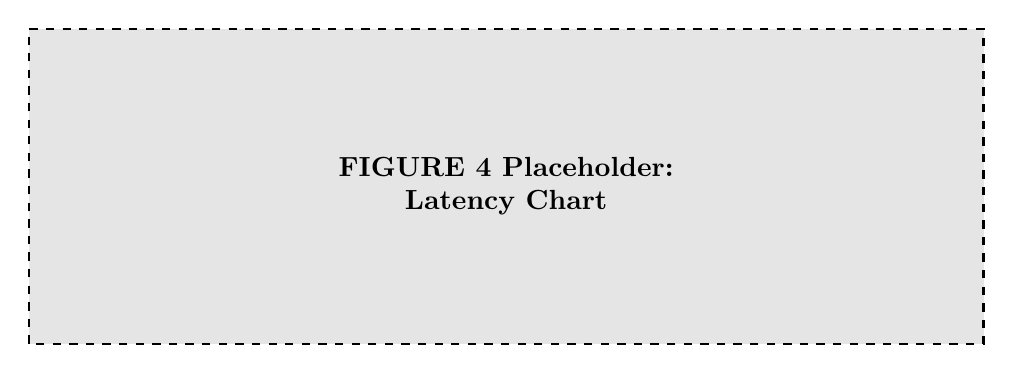
\begin{tikzpicture}
  \draw[thick, dashed, fill=gray!20] (0,0) rectangle (\columnwidth, 4cm);
  \node[align=center] at (0.5\columnwidth, 2cm) {\textbf{FIGURE 4 Placeholder:} \\ \textbf{Latency Chart}};
\end{tikzpicture}
\caption{Expected wall clock latency comparison between LLM as a judge alignment (1.68s) and our distilled late interaction student model (milliseconds), to be measured with batch size $G=8$.}
\label{fig:placeholder}
\end{figure}

\subsection{Reasoning Alignment and Breakpoint Fidelity}

To confirm that our framework successfully aligns trajectories and detects logical errors, we plan to measure alignment fidelity across the test set.

\textbf{Metrics.} We will report alignment accuracy, measuring how often the target reasoning mode selected by $D_{\mathrm{align}}$ matches human expert judgements of strategic similarity.

\textbf{Causal Validation of Breakpoint Detection.} A critical potential vulnerability is whether semantic divergence merely detects stylistic shifts rather than genuine reasoning failure. To rigorously prove the causal link between trajectory divergence and logical invalidity, we will perform a controlled intervention experiment. We will inject controlled reasoning corruptions (e.g., swapping a single logical step while preserving the exact lexical style) into known correct trajectories. We hypothesize that the divergence spike will perfectly isolate the corrupted step. Conversely, we will cluster same answer trajectories by semantic distance to confirm that our topology alignment does not penalize valid semantic novelty, thereby suppressing hallucination without suppressing exploration.

\textbf{Evaluation protocol.} We will sample incorrect rollouts and map them to their corresponding $D_{\mathrm{align}}$ targets. Human annotators will evaluate if the target reasoning mode shares the same foundational algebraic strategy before the logical breakpoint occurred.

\subsection{Empirical Validation of Core Hypotheses}

Two analyses are designed to validate the theoretical assumptions underlying our framework.

\textbf{Student Distillation Convergence (Hypothesis 4a).} We will plot the validation loss curve of the student model across training epochs, tracking the MSE between student MaxSim scores and teacher deviation scores on the held out 5,000 pair validation set. We hypothesize that this curve will converge, demonstrating that the student successfully internalizes the capacity to measure logical deviation.

\textbf{Continuous Divergence Spikes (Hypothesis 4b).} We will plot the Divergence Vector $d_t$ against reasoning step index $t$ for a representative set of incorrect rollouts mapped to their target reasoning mode. We hypothesize that the continuous penalty weight generated by the sigmoid function will exhibit a sharp spike that perfectly coincides with the specific reasoning steps at which the model introduces human-annotated logical errors. This will be rigorously evaluated using quantitative metrics, including Pearson correlation between divergence spikes and error positions, the AUROC for breakpoint detection, and a calibration curve to map continuous alignment scores to empirical logical failure probabilities.

Table~\ref{tab:casestudy} illustrates a representative case: a six-step algebra problem in which the student model assigns low $d_t$ (well below $\tau$) to the four correct foundational steps, then exhibits a sharp divergence spike at Step~5 upon an arithmetic error, confirming the causal link between topological departure and logical invalidity.

\begin{table}[htbp]
\centering
\small
\caption{
Case study: per-step divergence $d_t$ on a representative
incorrect rollout ($\tau = 0.50$, $\beta = 8$).
}
\label{tab:casestudy}

\begin{tabularx}{\linewidth}{c X c c c}
\toprule
\textbf{Step} &
\textbf{Reasoning content (abridged)} &
\boldmath$d_t$ &
\textbf{Status} &
\textbf{Penalty} \\
\midrule

1 &
Let $x$ be the unknown; equation: $2x+5=13$. &
0.08 &
\textcolor{blue!80!black}{$\checkmark$} &
$\approx 0$ \\

2 &
Subtract 5: $2x = 8$. &
0.11 &
\textcolor{blue!80!black}{$\checkmark$} &
$\approx 0$ \\

3 &
Divide by 2: $x = 4$. &
0.09 &
\textcolor{blue!80!black}{$\checkmark$} &
$\approx 0$ \\

4 &
Verify: $2(4)+5 = 13$. &
0.13 &
\textcolor{blue!80!black}{$\checkmark$} &
$\approx 0$ \\

\rowcolor{red!12}
5 &
\textbf{Compute $2+3=6$ (arithmetic error).} &
\textbf{0.74}$\uparrow$ &
\textcolor{red!80!black}{$\times$} &
sigmoid amp. \\

\rowcolor{red!12}
6 &
Therefore $x = 6/2 = 3$ (wrong conclusion). &
0.81 &
\textcolor{red!80!black}{$\times$} &
sigmoid amp. \\

\bottomrule
\end{tabularx}

\vspace{2pt}
\footnotesize
Steps 1--4: $d_t < \tau$ $\Rightarrow$
Preservation Zone, gradient $\approx 0$.
Step 5: $d_t \gg \tau$ $\Rightarrow$
sigmoid-amplified penalty activated.

\end{table}

\textbf{Uncertainty Calibration (Hypothesis 4c).} To prove that our continuous alignment scores reliably map to empirical failure probabilities, we will plot Reliability Diagrams and compute the Expected Calibration Error and Brier Score. This establishes our alignment metric as a rigorously calibrated uncertainty field rather than a heuristic confidence weight.

\textbf{Empirical Stability Analysis under Policy Coupled Masking (Hypothesis 4d).} Because the generation of the advantage mask depends on the policy itself, the estimator is policy coupled. To ensure this does not induce severe RL instability, we will conduct an empirical stability analysis tracking four critical metrics across training steps: Gradient Norm Variance (measuring optimization stability), KL Drift (measuring policy stability), Entropy Collapse (measuring exploration retention), and Reward Variance (measuring the masking effect).

\textbf{Reasoning Manifold and Uncertainty Visualizations.} We will generate UMAP and t SNE projections to visualize the dynamic reasoning manifold, illustrating the separation between correct and incorrect trajectories. Additionally, we will provide visualizations of token level uncertainty spikes over the Chain of Thought, explicit breakpoint visualization showing exactly where reasoning collapses, and plots depicting cluster evolution during the online reinforcement learning process.

\begin{figure*}[htbp]
\centering
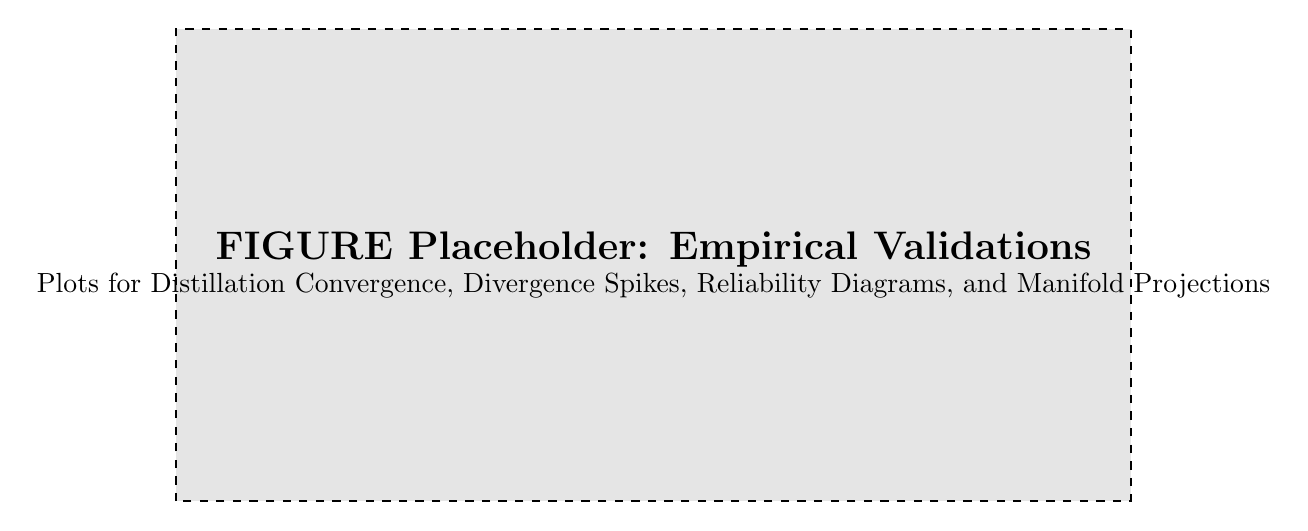
\begin{tikzpicture}
  \draw[thick, dashed, fill=gray!20] (0,0) rectangle (\textwidth, 6cm);
  \node[align=center] at (0.5\textwidth, 3cm) {\Large \textbf{FIGURE Placeholder: Empirical Validations} \\ Plots for Distillation Convergence, Divergence Spikes, Reliability Diagrams, and Manifold Projections};
\end{tikzpicture}
\caption{Empirical validation results for the core hypotheses.}
\label{fig:empirical_validation}
\end{figure*}



% -------------------------------------------------------
\section{Proposed Ablation Studies}
% -------------------------------------------------------

To isolate the contribution of each major design choice, we design four ablation studies to be conducted as part of the proposed experimental protocol.

\subsection{Alignment Target Selection Strategy}

To validate our core strategy of aligning with the consensus anchored correct trajectories rather than the group average, we will compare three advantage modulation configurations:

\begin{itemize}
    \item \textbf{Config A Vanilla GRPO:} Advantage is applied uniformly to all tokens in the sequence regardless of trajectory divergence.
    \item \textbf{Config B Average Group Alignment:} The per token divergence signal used to compute the sigmoid penalty is derived from the distance between the incorrect rollout and the average embedding of all other rollouts in the group. This represents a noisy, non targeted diversity penalization approach.
    \item \textbf{Config C Consensus Anchored Alignment (Ours):} The per token divergence signal is derived strictly from $d_t$ computed against the closest valid reasoning mode $C_{\mathrm{target}}$ identified from consensus anchored correct trajectories.
\end{itemize}

We expect that Config C will achieve the highest Pass@1 on MATH500. We hypothesize that aligning with the average group embedding (Config B) will yield noisy divergence signals, because the group average may incorporate other incorrect or semantically unrelated paths. Aligning exclusively with the consensus anchored correct trajectories (Config C) guarantees that the divergence score $d_t$ measures true logical departure from a valid reasoning strategy, producing accurate soft penalties that protect foundational steps while suppressing hallucination zones.

\subsection{Step-level vs. Sequence-level Credit Assignment}

We will ablate our Advantage Mask $\hat{A}_{i,t}$ by comparing two granularities of credit assignment:

\begin{itemize}
    \item \textbf{Sequence level penalty (baseline):} A single scalar modifier derived from $D_{\mathrm{align}}$ is applied uniformly to all tokens in the sequence. This is equivalent to the approach taken by Vanilla GRPO and SEED GRPO, which do not distinguish between foundational reasoning steps and divergence points.
    \item \textbf{Sigmoid continuous masking (ours):} The per token divergence vector $\mathbf{d}_t$ retained from the MaxSim intermediate scores is fed into the sigmoid soft penalty (Equation 4). Steps with low divergence receive near zero penalty, while steps crossing the threshold $\tau$ are amplified continuously. This formulation is fully differentiable and eliminates the brittleness of a hard cutoff.
\end{itemize}

We will measure convergence speed (accuracy at training steps 500, 1000, 2000) and final Pass@1 on MATH500. We additionally plan to track performance on a held-out set of foundational reasoning tasks to test whether sequence-level penalization degrades basic reasoning competence - a form of catastrophic forgetting that step-level masking is designed to prevent by shielding high-certainty early steps from unnecessary gradient interference.

\subsection{Continuous Trajectory Alignment vs Discrete Semantic Entropy}

This ablation will directly test the information quality of our continuous alignment signal against discrete clustering approaches. We will replace our trajectory alignment score $D_{\mathrm{align}}$ with Discrete Semantic Entropy computed by clustering the $G$ rollouts into $K$ semantic clusters based on final answers, then computing Shannon entropy over cluster assignments.

\begin{itemize}
    \item \textbf{Discrete SE:} Rollouts are clustered into $K$ groups by final answer. Uncertainty is the Shannon entropy over cluster proportions.
    \item \textbf{Continuous Trajectory Alignment (ours):} The penalty is derived from $D_{\mathrm{align}}$, the asymmetric matching distance to the closest correct trajectory computed by the distilled late interaction model.
\end{itemize}

We will evaluate both variants on two problem subsets: short chain of thought problems and long chain of thought problems. We hypothesize that the performance gap between $D_{\mathrm{align}}$ and discrete entropy will widen significantly on the long chain of thought subset, confirming that discrete clustering is structurally ill suited for process level reasoning evaluation.

\subsection{Hyperparameter Sensitivity}

We will evaluate the robustness of our method to its key hyperparameters. All sensitivity experiments will be run on MATH500 with Pass@1 as the evaluation metric.

\textbf{Soft penalty parameters $\tau$, $\alpha$, and $\beta$.} We will systematically ablate the parameters governing our continuous sigmoid advantage mask. We will tune $\tau$ (the sensitivity threshold), $\alpha$ (the penalty amplification intensity), and $\beta$ (the sharpness of the sigmoid slope) to identify the optimal equilibrium between protecting foundational knowledge and punishing hallucinations.

\textbf{Number of rollouts $G$.} We will evaluate $G \in \{8, 10, 16\}$. A key advantage of our late interaction distillation is its minimal computational complexity. We will report both Pass@1 accuracy and per batch wall clock time for each $G$, with the goal of demonstrating that larger rollout groups yield more reliable correct alignment targets without incurring prohibitive latency overhead.

% -------------------------------------------------------
\section{Limitations}
% -------------------------------------------------------

Lexical invariance limits. Our step level divergence estimation relies on implicit token boundary alignment between reasoning trajectories. Although distilling from an LLM Judge significantly mitigates lexical noise compared to standard embeddings, it does not yet achieve perfect semantic invariance. For free form chains of thought that do not naturally decompose into discrete logical steps, the Divergence Vector may still capture some surface level lexical differences.

Aggregation gap in distillation. Although late-interaction architectures empirically produce reliable token-level alignments~\cite{b10}, our MSE loss is computed over a scalar topology cost. This formulation cannot theoretically guarantee the absence of token-level compensation during training. Future work could explore contrastive token-level distillation to provide strict mathematical bounds on local divergence estimation.

Alignment induced novelty suppression. While aligning with correct trajectories mitigates hallucination, it carries an intrinsic risk of forcing reasoning paths to converge toward the most common solution strategy, potentially suppressing the emergence of valid but idiosyncratic reasoning strategies.

Gradient bias from advantage modulation. While our token level re normalization step recovers the unbiased property of the baseline advantage estimator, we do not provide a theoretical guarantee of global optimality under arbitrary non stationary reward distributions. Because the masking generation itself is a policy dependent transformation, the gradient estimator may still contain a potential hidden bias. The convergence behavior under extreme variance remains an open question for future theoretical analysis.

Domain generalization. The framework is designed and evaluated on mathematical reasoning, where reasoning steps are well defined and verifiable. Generalization to open ended domains such as commonsense reasoning, code generation, or multi modal tasks is not validated in this work and may require domain specific adaptations to the step alignment strategy.

Failure Mode Taxonomy. We will conduct an honest failure analysis by categorizing unhandled rollouts into a strict taxonomy: Type A (Semantic divergence but logical correctness, identifying exploration drift), Type B (Lexical similarity but hidden logical error, identifying masking failures), Type C (Late stage reasoning collapse), and Type D (Exploration drift where the policy abandons the target reasoning mode). This transparent taxonomy will identify boundaries where topological alignment degrades.

Offline distillation data dependency. The quality of the distilled student model depends on the coverage and diversity of the offline training set. Distribution shift between this training set and the online task may degrade the accuracy of divergence estimation for out of distribution prompts, particularly for competition level problems that are underrepresented in the distillation data.

Distribution shift of reasoning trajectories. Although the student model learns a robust logical distance metric from the LLM Judge, its offline distillation relies on a static dataset of reasoning pairs. As the policy optimizes and explores during the online RL phase, it may generate highly novel reasoning structures or out-of-distribution (OOD) logical errors that were underrepresented in the offline distillation phase. Over time, as the policy's output distribution shifts away from the offline dataset, the continuous divergence scores produced by the static student model may become less calibrated. As a practical mitigation, we propose periodic re-distillation checkpoints: every $K$ training steps, the student model is briefly fine-tuned on a small buffer of recent rollout pairs annotated by the LLM Judge to track the evolving policy distribution. Evaluating the frequency and effectiveness of this mitigation is a key goal of our future empirical validation.

% -------------------------------------------------------
\section{Conclusion}
% -------------------------------------------------------

This work demonstrates that the computational bottleneck of process level diversity metrics need not be a barrier to their deployment in online reinforcement learning. By separating the expensive divergence computation into an offline distillation phase, we recover the structural richness of trajectory divergence at the latency of a single encoder forward pass.

Empirically, our proposed experiments are designed to validate the core hypotheses of the framework: that distillation loss converges, that the per token divergence signal correctly identifies logical failure zones, and that the soft advantage mask produces superior Pass@1 and Pass@$k$ scores relative to baselines across MATH500 and GSM8K.

The immediate future work will focus on executing the proposed experimental protocol to empirically validate the latency reduction and accuracy gains across mathematical reasoning benchmarks. This includes verifying the core hypotheses, namely that distillation loss converges and that divergence spikes co occur with reasoning errors, as well as conducting the full ablation studies to isolate the contribution of each design choice. Longer term work will address the theoretical gradient properties of step level advantage masking and explore the generalization of this framework beyond mathematical reasoning to broader multi step reasoning domains.

\section*{Acknowledgment}
We use large language models strictly for language polishing, grammatical corrections, and improving the clarity of the text during the preparation of this manuscript. We reviewed, edited, and take full responsibility for the entirety of the scientific content and originality of this work.

\begin{thebibliography}{00}
\bibitem{b1} M. Chen et al., SEED GRPO: Semantic entropy enhanced GRPO for uncertainty aware policy optimization, arXiv preprint arXiv:2505.12346, 2025.
\bibitem{b2} Z. Shao et al., DeepSeekMath: Pushing the Limits of Mathematical Reasoning in Open Language Models, arXiv preprint arXiv:2402.03300, 2024.
\bibitem{b3} G. Hinton et al., Distilling the Knowledge in a Neural Network, arXiv preprint arXiv:1503.02531, 2015.
\bibitem{b4} V. Sanh et al., DistilBERT, a distilled version of BERT, arXiv preprint arXiv:1910.01108, 2019.
\bibitem{b5} X. Jiao et al., TinyBERT: Distilling BERT for Natural Language Understanding, EMNLP 2020.
\bibitem{b6} N. Ho et al., Large Language Models are Reasoning Teachers, ACL 2023.
\bibitem{b7} H. Lightman et al., Let's Verify Step by Step, arXiv preprint arXiv:2305.20050, 2023.
\bibitem{b8} P. Wang et al., Math Shepherd: Verify and Reinforce LLMs Step by step without Human Annotations, ACL 2024.
\bibitem{b9} D. M. Ziegler et al., Fine Tuning Language Models from Human Preferences, arXiv preprint arXiv:1909.08593, 2019.
\bibitem{b10} L. Santos et al., ColBERTv2: Effective and Efficient Retrieval via Lightweight Late Interaction, NAACL 2022.
\bibitem{b11} J. Schulman et al., Proximal Policy Optimization Algorithms, arXiv preprint arXiv:1707.06347, 2017.
\bibitem{b12} DeepSeek-AI, DeepSeek-R1: Incentivizing Reasoning Capability in LLMs via Reinforcement Learning, arXiv preprint arXiv:2501.12948, 2025.
\bibitem{b13} C. Yu et al., DAPO: An Open Source LLM Reinforcement Learning System at Scale, arXiv preprint arXiv:2503.14476, 2025.
\bibitem{b14} J. Luo et al., OmegaPRM: Improving Process Reward Model Training with Divide and Conquer Monte Carlo Tree Search, arXiv preprint arXiv:2408.06643, 2024.
\end{thebibliography}

\end{document}